\documentclass{article}
\usepackage{amsmath}
\usepackage[margin=1in]{geometry}
\usepackage{amsfonts}
\usepackage{hyperref}
\usepackage{graphicx}

\begin{document}
	
\title{Linear Combination}
\author{Andy Chong Sam}

\maketitle	

\section{Linear Combinations Visual Intution}
\begin{minipage}[c]{.5\linewidth}
	\par \noindent We first start with the idea of a generic vector which can be scaled by a positive or negative k. As seen on Figure 1, given positive enough or negative values of k, the vector can occupy a line of space.
\end{minipage}%%%
\begin{minipage}[c]{.5\linewidth}
\begin{center}
	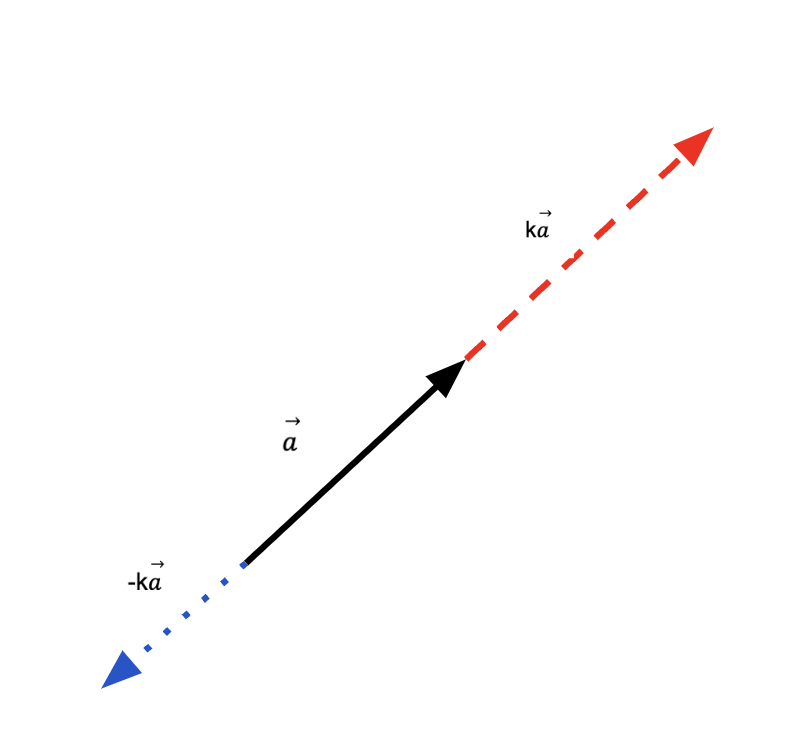
\includegraphics[width=3cm]{matrix-scaling-1.png}
\end{center}
\begin{center}
	Figure 1	
\end{center}
\end{minipage}
\linebreak
\linebreak
\linebreak
\begin{minipage}[c]{.5\linewidth}
	\par \noindent Now suppose we have two vectors \( \vec a \) and \( \vec b \).  They can each be scaled independently. Both vectors can also be added together. With some visual imagination we how by varying the scaling factor of each vector we can reach every point on the two dimensional plane.
\end{minipage}%%%
\begin{minipage}[c]{.5\linewidth}
\begin{center}
	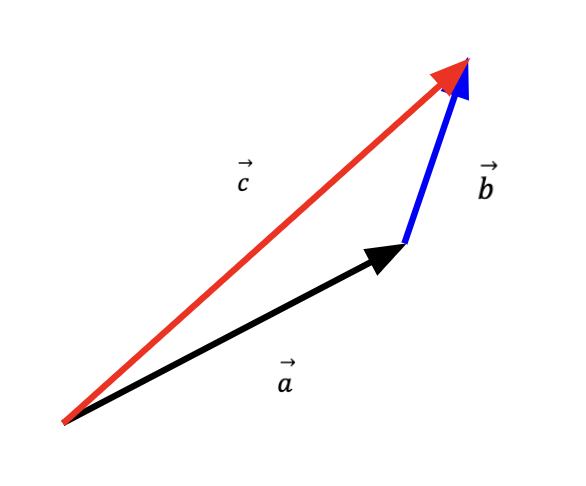
\includegraphics[width=3cm]{vector-scaling-2.png}
\end{center}
\begin{center}
	Figure 2	
\end{center}
\end{minipage}
\linebreak
\linebreak
\linebreak
\begin{minipage}[c]{.5\linewidth}
	\par \noindent We can of course add multiple vectors together, each with the ability to scale independently. A hypothetical situation with three vectors is shown on Figure 3.
\end{minipage}%%%
\begin{minipage}[c]{.5\linewidth}
\begin{center}
	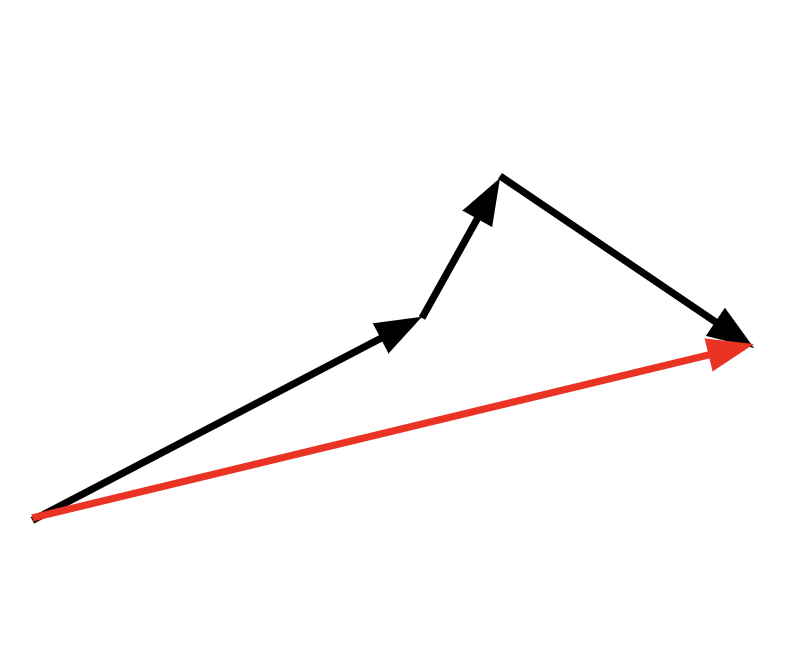
\includegraphics[width=3cm]{matrix-scaling-3.png}
\end{center}
\begin{center}
	Figure 3
\end{center}
\end{minipage}
\newline
\newline
\newline
\par \noindent We can describe describe the summation of n vectors \(<x_n, y_n>\) together like so:
\[
k_1
\left(\begin{array}{@{}c@{}}
	x_1 \\
	y_1 \\
\end{array}\right) + 
k_2
\left(\begin{array}{@{}c@{}}
	x_2 \\
	y_2 \\
\end{array}\right) + 
k_3
\left(\begin{array}{@{}c@{}}
	x_3 \\
	y_3 \\
\end{array}\right) + 
... 
k_n
\left(\begin{array}{@{}c@{}}
	x_n \\
	y_n \\
\end{array}\right) =
\left(\begin{array}{@{}c@{}}
	k_1 x_1 + k_2 x_2 + ... + k_n x_n \\
	k_1 y_1 + k_2 y_2 + ... + k_n y_n \\
\end{array}\right) 
\]
\par \noindent The expression above can be rewritten in the form of a matrix multiplication:
\[
\left(\begin{array}{@{}cccc@{}}
	x_1 & x_2 & ... &x_n\\
	y_1 & y_2 & ... &y_n\\
	
\end{array}\right) 
\left(\begin{array}{@{}c@{}}
	k_1 \\
	k_2 \\
	... \\
	k_n
\end{array}\right) 
\]
\par \noindent It is for this reason that when vectors are written into a matrix they are often done so vertically down a column.

\par \noindent Problems related to linear combinations involve verifying if a vector is a combination of other vectors. A few examples are provided below.
\newline
\newline
\framebox{
	\parbox{\linewidth}
	{
		\par\noindent Write \(<12,10>\) as a linear combination of \(<2,2>\) and \(<1,3>\).
		\newline
		\par\noindent We want to solve for the matrix \(<k_1, k_2>\):
		\[
			\left(\begin{array}{@{}cc@{}}
				2 & 3\\
				2 & 1\\
			\end{array}\right) 
			\left(\begin{array}{@{}c@{}}
				k_1\\
				k_2\\
			\end{array}\right) =
			\left(\begin{array}{@{}c@{}}
				10\\
				12\\
			\end{array}\right)	
		\]
		\par\noindent Which can be solved with the augmented matrix:
		\[
			\left(\begin{array}{@{}cc|c@{}}
				2 & 3 & 10\\
				2 & 1 & 12\\
			\end{array}\right) 
		\]
		\[
			\left(\begin{array}{@{}cc|c@{}}
				2 & 3 & 10\\
				2 & 1 & 12\\
				\end{array}\right)
			\xrightarrow[]{R_2 - R_1 = R_2} 	
			\left(\begin{array}{@{}cc|c@{}}
				2 & 3 & 10\\
				0 & -2 & 2\\
			\end{array}\right)	
			\xrightarrow[]{-\frac{1}{2}R_2 = R_2} 
			\left(\begin{array}{@{}cc|c@{}}
				2 & 3 & 10\\
				0 & 1 & -1\\
			\end{array}\right)		
			\xrightarrow[]{-\frac{1}{2}R_1 = R_1}							
		\]
		\[
		\left(\begin{array}{@{}cc|c@{}}
			1 & \frac{3}{2} & 5\\
			0 & 1 & -1\\
		\end{array}\right)
		\xrightarrow[]{R_1 - \frac{3}{2}R_2 = R_1}	
			\left(\begin{array}{@{}cc|c@{}}
			1 & 0 & \frac{13}{2}\\
			0 & 1 & -1\\
			\end{array}\right)		
		\]
		\newline
		\par\noindent \textbf{Solution:}
		\[
		 \frac{13}{2}
		\left(\begin{array}{@{}c@{}}
			2 \\
			2 \\
		\end{array}\right) -
		\left(\begin{array}{@{}c@{}}
		3 \\
		1 \\
		\end{array}\right)		
		=
		\left(\begin{array}{@{}c@{}}
			10\\
			12\\
		\end{array}\right)\]
	}
}
\newline
\newline
\newline
\framebox{
	\parbox{\linewidth}
	{
		\par\noindent Write \(<-5,3,16>\) as a linear combination of \(<1, -1, 4>\) and \(<-3, 2, 6>\).
		\newline
		\par \noindent We proceed to setup the augmented matrix and reduce:
		\newline
		\[
		\left(\begin{array}{@{}cc|c@{}}
			1 & -3 & -5\\
			-1 & 2 & 3\\
			4 & 6 & 16 \\
		\end{array}\right)
		\xrightarrow[]{R_2 <--> R_3}	
		\left(\begin{array}{@{}cc|c@{}}
			1 & -3 & -5\\
			4 & 6 & 16 \\
		    -1 & 2 & 3\\
		\end{array}\right)
		\xrightarrow[]{\frac{1}{2}R_2 = R_2}	
		\left(\begin{array}{@{}cc|c@{}}
			1 & -3 & -5\\
			2 & 3 & 8 \\
			-1 & 2 & 3\\
		\end{array}\right)
		\xrightarrow[]{R_1 + R_2 = R_1}	
		\]
		\newline
		\[
		\left(\begin{array}{@{}cc|c@{}}
			3 & 0 & 3\\
			2 & 3 & 8\\
			-1 & 2 & 3 \\
		\end{array}\right)
		\xrightarrow[]{\frac{1}{3}R_1 = R_1}	
		\left(\begin{array}{@{}cc|c@{}}
			1 & 0 & 1\\
			2 & 3 & 8 \\
			-1 & 2 & 3\\
		\end{array}\right)
		\xrightarrow[]{R_2 - 2R_1 = R_2}	
		\left(\begin{array}{@{}cc|c@{}}
			1 & 0 & 1\\
			0 & 3 & 6 \\
			-1 & 2 & 3\\
		\end{array}\right)
		\xrightarrow[]{\frac{1}{3}R_2 = R_2}	
		\]
		\newline
		\[
		\left(\begin{array}{@{}cc|c@{}}
			1 & 0 & 1\\
			0 & 1 & 2\\
			-1 & 2 & 3 \\
		\end{array}\right)
		\xrightarrow[]{R_3 + R_1 = R_3}	
		\left(\begin{array}{@{}cc|c@{}}
			1 & 0 & 1\\
			0 & 1 & 2 \\
			0 & 2 & 4\\
		\end{array}\right)
		\xrightarrow[]{R_3 - 2R_2 = R_3}	
		\left(\begin{array}{@{}cc|c@{}}
			1 & 0 & 1\\
			0 & 1 & 2 \\
			0 & 0 & 0\\
		\end{array}\right)	
		\]
		\newline
		\par\noindent \textbf{Solution:} 
		\[
		\left(\begin{array}{@{}c@{}}
			1 \\
		   -1 \\
			4
		\end{array}\right) +
		2\left(\begin{array}{@{}c@{}}
			-3 \\
			2 \\
			6
		\end{array}\right)		
		=
		\left(\begin{array}{@{}c@{}}
			-5\\
			3\\
			16
		\end{array}\right)\]
}}
\newpage
\section{Linear Independence}
\par\noindent If a vector can be obtained by scaling another vector, then the two vectors are dependent. A set of vectors is dependent if there exists \( c_1 ... c_n\) such that \(c_1v_1 + ... c_nv_n = 0\). If the only solution is the trivial solution \(c_1 = ... c_n = 0\), then the set is independent. 
\newline
\begin{minipage}[c]{.5\linewidth}
	\par \noindent Suppose we have \( \vec a = <1,1>\) and \( \vec b = <2,2>\) as shown on Figure 4. Since \( 2\vec a = \vec b\), we know that set \( \{ \vec a, \vec b\}\) is dependent.
\end{minipage}%%%
\begin{minipage}[c]{.5\linewidth}
	\begin{center}
		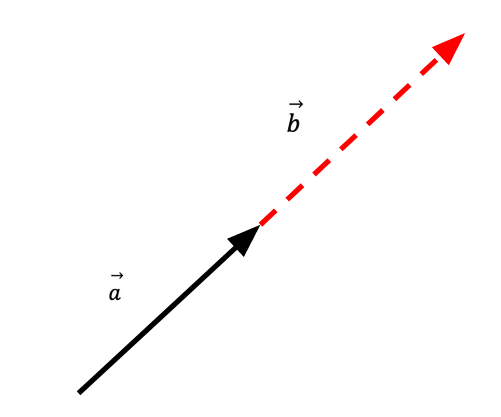
\includegraphics[width=3cm]{linear-combo.png}
	\end{center}
	\begin{center}
		Figure 4
	\end{center}
\end{minipage}
\newline
\par\noindent One possible intution is as follows. Suppose that there are two vectors \(v_1\) and \(v_2\). Based on our earlier definition, we know that if either vector can be scaled to obtain the other, then the set is not independent. If the set is dependent, then there is a constant \(k\) by which \(kv_2 = v_1\) or \(kv_1 = v_2\). In the latter case, we end up with \(kv_1 - v_2 = 0\). In this very specific example, the coefficient for \(v_2\) turned out to be negative, but we can generalize this whole expression to a general coefficient \(k_2\) which can be either positive or negative: \(k_1v_1 + k_2V_2 = 0\).
\newline
\par \noindent Here are some example problems:
\newline
\newline
\framebox{
	\parbox{\linewidth}
	{
	\par\noindent Determine if the set of vectors \(<2,2>\) and \(<-1,5>\) are independent or dependent.
	\newline
	\par\noindent We are solving for the matrix \(<k_1, k_2>\):
	\[
	\left(\begin{array}{@{}cc@{}}
		2 & -1 \\
		2 &  5 \\
	\end{array}\right)
\left(\begin{array}{@{}c@{}}
	k_1 \\
	k_2 \\
\end{array}\right)
	 = 
\left(\begin{array}{@{}c@{}}
	0 \\
	0 \\
\end{array}\right)	
\]
\[
	\left(\begin{array}{@{}cc|c@{}}
	2 & -1 & 0\\
	2 &  5 & 0 \\
\end{array}\right)
\xrightarrow[]{R_1 - \frac{1}{2}R_2 = R_2}
	\left(\begin{array}{@{}cc|c@{}}
	1 & -\frac{7}{2} & 0\\
	2 &  5 & 0 \\
\end{array}\right)
\xrightarrow[]{R_2 - 2R_1 = R_2}
	\left(\begin{array}{@{}cc|c@{}}
	2 & -\frac{7}{2} & 0\\
	0 &  12 & 0 \\
\end{array}\right)
\xrightarrow[]{\frac{1}{12}R_2 = R_2}
\]
\[
	\left(\begin{array}{@{}cc|c@{}}
	2 & -\frac{7}{2} & 0\\
	0 &  1 & 0 \\
\end{array}\right)
\xrightarrow[]{R_1 + \frac{7}{2}R_2 = R_1}
\left(\begin{array}{@{}cc|c@{}}
	1 &  0 & 0\\
	0 &  1 & 0 \\
\end{array}\right)
\]
\[
\left(\begin{array}{@{}c@{}}
	k_1 \\
	k_2 \\
\end{array}\right) = 
\left(\begin{array}{@{}c@{}}
	0 \\
	0 \\
\end{array}\right)
\]
\par\noindent \textbf{The set is independent}.
}
}
\newline
\newline
\newline
\framebox{
	\parbox{\linewidth}
	{
		\par\noindent Determine if the set of vectors \(<-1,4>\) and \(<2,-8>\) are independent or dependent.
		\newline
		\par\noindent We are solving for the matrix \(<k_1, k_2>\):
		\[
		\left(\begin{array}{@{}cc@{}}
			-1 & 2 \\
			4 &  -8 \\
		\end{array}\right)
		\left(\begin{array}{@{}c@{}}
			k_1 \\
			k_2 \\
		\end{array}\right)
		= 
		\left(\begin{array}{@{}c@{}}
			0 \\
			0 \\
		\end{array}\right)	
		\]
		\[
		\left(\begin{array}{@{}cc|c@{}}
			-1 & 2 & 0\\
			4 &  -8 & 0 \\
		\end{array}\right)
		\xrightarrow[]{R_1 <--> R_2}
		\left(\begin{array}{@{}cc|c@{}}
			4 & -8 & 0\\
			-1 & 6 & 0 \\
		\end{array}\right)
		\xrightarrow[]{R_1 + 3R_2 = R_1}
		\left(\begin{array}{@{}cc|c@{}}
			1 & -2 & 0\\
			-1 & 2 & 0 \\
		\end{array}\right)
		\xrightarrow[]{R_2 + R_1 = R_2}
		\left(\begin{array}{@{}cc|c@{}}
			1 & -2 & 0\\
			0 &  0 & 0 \\
		\end{array}\right)
		\]		
		\par\noindent We are left with \(k_1 - 2k_2 = 0\), or \(k_1 = 2k_2\). Any combination of \(k_1\) and \(k_2\) that meet the established relationship will work, hence there are solutions other than the trivial solution.
		\newline
		\par\noindent \textbf{The set is dependent.}
	}
}
\newpage
\par\noindent Here are some examples using vectors with three components:
\newline
\framebox{
	\parbox{\linewidth}
	{
		\par\noindent Determine if the set of vectors \(<1,2,3>\) , \(<-2,1,0>\), and \(<1,0,1>\) are independent or dependent.
		\newline
		\par\noindent We are solving for the matrix \(<k_1, k_2, k_3>\):
		\[
			\left(\begin{array}{@{}ccc@{}}
				1 & -2 & 1 \\
				2 &  1 & 0 \\
				3 & 0 & 1 \\
			\end{array}\right)
			\left(\begin{array}{@{}c@{}}
				k_1 \\
				k_2 \\
				k_3 \\
			\end{array}\right)
			= 
			\left(\begin{array}{@{}c@{}}
				0 \\
				0 \\
				0 \\
			\end{array}\right)	
			\]	
			\[
			\left(\begin{array}{@{}ccc|c@{}}
				1 & -2 & 1 & 0\\
				2 &  1 & 0 & 0 \\
				3 & 0 & 1 & 0  \\
			\end{array}\right)
			\xrightarrow[]{R_2 - 2R_1 = R_2}
			\left(\begin{array}{@{}ccc|c@{}}
				1 & -2 & 1 & 0\\
				0 &  5 & -2 & 0 \\
				3 & 0 & 1 & 0  \\
			\end{array}\right)
			\xrightarrow[]{\frac{1}{5}R_2 = R_2}
			\left(\begin{array}{@{}ccc|c@{}}
				1 & -2 & 1 & 0\\
				0 &  1 & \frac{2}{5} & 0 \\
				3 & 0 & 1 & 0  \\
			\end{array}\right)
			\xrightarrow[]{R_3 - 3R_1 = R_3}
			\]
			\[
			\left(\begin{array}{@{}ccc|c@{}}
				1 & -2 & 1 & 0\\
				0 &  1 & \frac{2}{5} & 0 \\
				0 & 6 & -2 & 0  \\
			\end{array}\right)
			\xrightarrow[]{R_3 - 6R_2 = R_3}
			\left(\begin{array}{@{}ccc|c@{}}
				1 & -2 & 1 & 0\\
				0 &  1 & \frac{2}{5} & 0 \\
				0 & 0 & \frac{2}{5} & 0  \\
			\end{array}\right)
		\xrightarrow[]{R_2+R_3=R_2}
			\left(\begin{array}{@{}ccc|c@{}}
			1 & -2 & 1 & 0\\
			0 &  1 & 0 & 0 \\
			0 & 0 & \frac{2}{5} & 0  \\
		\end{array}\right)
		\xrightarrow[]{R_1+2R_2=R_1} \\
			\]
			\[
			\left(\begin{array}{@{}ccc|c@{}}
		1 & 0 & 1 & 0\\
		0 &  1 & 0 & 0 \\
		0 & 0 & \frac{2}{5} & 0  \\
	\end{array}\right)
	\xrightarrow[]{\frac{5}{2}R_3 = R_3}
	\left(\begin{array}{@{}ccc|c@{}}
		1 & 0 & 1 & 0\\
		0 &  1 & 0 & 0 \\
		0 & 0 & 1 & 0  \\
	\end{array}\right)		
		\]
		\[
		\left(\begin{array}{@{}c@{}}
			k_1 \\
			k_2 \\
			k_3 \\
		\end{array}\right) = 
		\left(\begin{array}{@{}c@{}}
		0 \\
		0 \\
		0 \\
		\end{array}\right)		
		\]
		\par\noindent \textbf{The set is independent.}
	}
}
\newline
\newline
\newline
\framebox{
	\parbox{\linewidth}
	{
		\par\noindent Determine if the set of vectors \(<1,0,1>\) , \(<1,1,0>\), and \(<0,1,-1>\) are independent or dependent.
		\newline
		\par\noindent We are solving for the matrix \(<k_1, k_2, k_3>\):
		\[
		\left(\begin{array}{@{}ccc@{}}
			1 & 1 & 0 \\
			0 & 1 & 1 \\
			1 & 0 & 1 \\
		\end{array}\right)
		\left(\begin{array}{@{}c@{}}
			k_1 \\
			k_2 \\
			k_3 \\
		\end{array}\right)
		= 
		\left(\begin{array}{@{}c@{}}
			0 \\
			0 \\
			0 \\
		\end{array}\right)	
		\]	
		\[
		\left(\begin{array}{@{}ccc|c@{}}
			1 & 1 & 0 & 0\\
			0 & 1 & 1 & 0 \\
			1 & 0 & -1 & 0  \\
		\end{array}\right)
		\xrightarrow[]{R_1 - 2R_2 = R_1}
		\left(\begin{array}{@{}ccc|c@{}}
			1 & 0 & -1 & 0\\
			0 & 1 & 1 & 0 \\
			1 & 0 & -1 & 0  \\
		\end{array}\right)
		\xrightarrow[]{R_3 - R_1 = R_3}
		\left(\begin{array}{@{}ccc|c@{}}
			1 & 0 & -1 & 0\\
			0 &  1 & 1 & 0 \\
			0 & 0 & 0 & 0  \\
		\end{array}\right)
		\]
		\par\noindent We are left with \(k_1 - k_3 = 0\) and \(k_2 + k_3 = 0\), or \(k_1 = k_3\) and \(k_2 = -k_3\). Any combination of \(k_1,k_2,k_3\) that meets the criteria is a possible solution.
		\newline
		\par\noindent \textbf{The set is dependent.}
	}
}
\newline
\end{document}